\iffalse
\documentclass[10pt,a4paper]{report}
%\usepackage[latin1]{inputenc}
\usepackage[utf8]{inputenc}
\usepackage{amsmath}
\usepackage{amsfonts}
\usepackage{amssymb}
\usepackage{graphicx}
\usepackage{multicol}
\usepackage{tabularx}
\usepackage{tikz}
\usetikzlibrary{arrows,shapes,automata,petri,positioning,calc}
\usepackage{hyperref}
\usepackage{tikz}
\usetikzlibrary{matrix,calc}
\usepackage[margin=0.5in]{geometry}
% ---- power functions -----% 
\newcommand{\myvec}[1]{\ensuremath{\begin{pmatrix}#1\end{pmatrix}}}
\let\vec\mathbf

\providecommand{\norm}[1]{\left\lVert#1\right\rVert}
\providecommand{\abs}[1]{\left\vert#1\right\vert}
\let\vec\mathbf

\newcommand{\mydet}[1]{\ensuremath{\begin{vmatrix}#1\end{vmatrix}}}
\providecommand{\brak}[1]{\ensuremath{\left(#1\right)}}
\providecommand{\lbrak}[1]{\ensuremath{\left(#1\right.}}
\providecommand{\rbrak}[1]{\ensuremath{\left.#1\right)}}
\providecommand{\sbrak}[1]{\ensuremath{{}\left[#1\right]}}
%-------end power functions----%
\newenvironment{Figure}
  {\par\medskip\noindent\minipage{\linewidth}}
  {\endminipage\par\medskip}
\begin{document}
%--------------------logo figure-------------------------%
\begin{figure*}[!tbp]
  \centering
  \begin{minipage}[b]{0.4\textwidth}
    
\includegraphics[scale = 0.5]{iitlogo.png}
  \end{minipage}
  \vspace{0.2cm}
\end{figure*}
%--------------------name & rollno-----------------------
\raggedright \textbf{Name}:\hspace{1mm} Ganga Gopinath\hspace{3cm} \Large \textbf{Assignment-6}\hspace{2.5cm} % 
\normalsize \textbf{Roll No.} :\hspace{1mm} FWC22050\vspace{1cm}
\begin{multicols}{2}

%----------------problem statement--------------%
\raggedright \textbf{Problem Statement:}\vspace{2mm}
\raggedright \\ 
\fi
	Find the area of the region bounded by the parabola $y=x^2$ and $y= \abs{x}$.
	\\
	\solution
	\begin{figure}[!h]
		\centering
 \includegraphics[width=\columnwidth]{chapters/12/8/1/9/figs/con3.pdf}
		\caption{}
		\label{fig:12/8/1/9}
  	\end{figure}
	\iffalse
\vspace{5mm}
%-----------------------------solution---------------------------
\raggedright \textbf{SOLUTION}:\vspace{2mm}\\

%---------given----------------%
\raggedright \textbf{Given}:\vspace{2mm}\\

Equation of Parabola is \\ \vspace{1mm}
\begin{align}
x^2=4y 
\end{align}
Equation of line is \\\vspace{1mm}
\begin{align}
y=|x|
\end{align}
From (1) we can say that Parabola is symmetric about the positive y axis.\\ \vspace{2mm}
%-------------To find ------------------%
\textbf{To Find }\vspace{2mm}\\
To find the intersection points and area of shaded region shown in figure\vspace{2mm}  \\ 
%--------------steps----------------------%
\textbf{STEP-1}\vspace{2mm}\\
The given parabola and line can be expressed as conics with parameters,\\ \vspace{1mm}

For Parabola,\\\vspace{1mm}
The conic parameters are
\begin{align}
\vec{V}_1=\myvec{
1 & 0\\
0 & 0
}
\end{align} 

\begin{align}
\vec{u_1}= -\myvec{
0\\
\frac{1}{2}
}\
\end{align} 
\begin{align}
f_1=0
\end{align} \vspace{2mm}

For line,\\\vspace{1mm}
\begin{align}
\vec{V}_2=\myvec{
0 & 0\\
0 & 0
}
\end{align} 


\begin{align}
\vec{u_2}= \myvec{
-\frac{1}{2}\\
\frac{1}{2}
}\
\end{align} 
\begin{align}
f_2=0
\end{align} \vspace{2mm}


\textbf{STEP-2}\vspace{2mm}\\
The points of intersection of the line is given by, \\ 
\begin{align}
L: \quad \vec{x} = \vec{q} + \kappa \vec{m} \quad \kappa \in \mathbb{R}
\end{align}
with the conic section, \\ 
\begin{align}
	\vec{x}^{\top}\vec{V}\vec{x} + 2\vec{u}^{\top} \vec{x} + f = 0
\end{align}
are given by \\
\begin{align}
\vec{x}_i = \vec{q} + \kappa_i \vec{m}
\end{align}
where, \\
{\tiny
\begin{multline}
\kappa_i = \frac{1}
{
\vec{m}^T\vec{V}\vec{m}
}
\lbrak{-\vec{m}^T\brak{\vec{V}\vec{q}+\vec{u}}}
\\
\pm
\rbrak{\sqrt{
\sbrak{
\vec{m}^T\brak{\vec{V}\vec{q}+\vec{u}}
}^2
-
\brak
{
\vec{q}^T\vec{V}\vec{q} + 2\vec{u}^T\vec{q} +f
}
\brak{\vec{m}^T\vec{V}\vec{m}}
}
}
\end{multline}
}
On substituting\\
\begin{align}
\vec{q} &= \myvec{
0\\
0.25
} 
\end{align}
\begin{align}
\vec{m} = \myvec{1 \\ 0}
\end{align}
With the given Parabola,\\ 
\begin{align}
	\vec{V} &= \myvec{
1 & 0\\
0 & 0
    }
\end{align}
\begin{align}
	\vec{u} = -\myvec{\frac{1}{2} \\0}
 \end{align}
 \begin{align}
  f = 0
 \end{align}
The value of $\kappa$ ,\\
\begin{align}
    \kappa = 1,-1
\end{align}
The points of intersection with Parabola along circle are \\
\begin{align}
    \vec{A}=\myvec{
1\\
1
    }
\end{align}
\begin{align}
    \vec{B}=\myvec{
-1\\
1
    }
\end{align}
\textbf{Result}
\begin{center}
 \includegraphics[width=0.5\textwidth]{con3.pdf}  
 \end{center}\vspace{1mm}
 From the figure,\\ \vspace{1mm}
Total area of portion is given by, \\ \vspace{1mm}
\begin{align}
 A=  \int_{0}^{1} g(x)-f(x) \,dx 
\end{align}
Where g(x) is area under line and f(x) is the area of parabola \\ \vspace{1mm}
\begin{align}
A= \int_{0}^{1} y dx -\int_{0}^{1} y_1 dx  \\
A= \int_{0}^{1} x dx -\int_{0}^{1} x^2 dx  \\
\end{align}
Area A is,\\ 
\begin{align}
    A= .333\,m^2
\end{align}
 \vspace{2mm} \textbf{Construction}
\begin{center}
\setlength{\arrayrulewidth}{0.5mm}
\setlength{\tabcolsep}{6pt}
\renewcommand{\arraystretch}{1.5}
    \begin{tabular}{|l|c|}
    \hline 
    \textbf{Points} & \textbf{coordinates} \\ \hline
   $\vec{A}$ & $\myvec{
   1\\
   1
   } $ \\ \hline
   $\vec{B}$ & $\myvec{
   -1\\
   1
   } $ \\\hline
      \end{tabular}
  \end{center}

\raggedright  Download the code \\
https://github.com/Gangagopinath/ASSIGNMENT/tree/
\newline
main/assignment6
  \end{multicols}
\end{document}
Footer
\fi
